\subsection{Semantic Web}


\begin{frame}
	\begin{block}{Semantic Web}
		% http://es.slideshare.net/rommelnc/probabilistic-ontology-representation-and-modeling-methodology-8647132
		\begin{quote}
			``The Semantic Web is an extension of the current web in which information is given well-defined meaning, better enabling computers and people to work in cooperation''~\cite{BernersLee01}
		\end{quote}
		\begin{itemize}
			\item Extension of the web through standards by W3C
			\item Change focus from data driven to knowledge driven
		\end{itemize}
	\end{block}
\end{frame}

\begin{frame}
	\begin{figure}
		\centering
		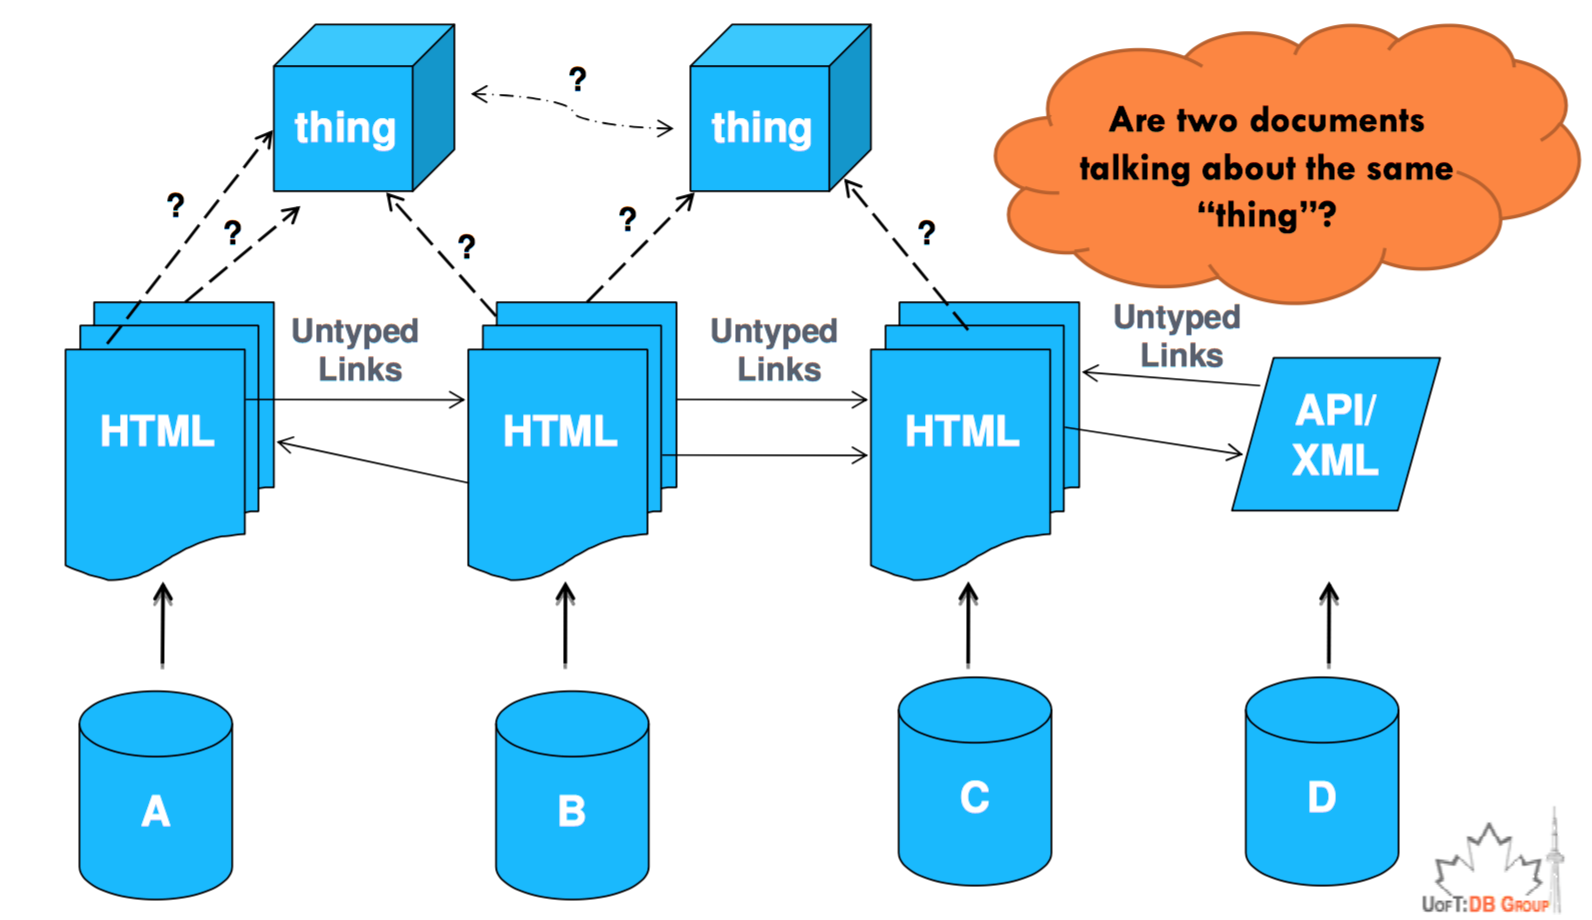
\includegraphics[width=\textwidth]{images/documentweb}
		\caption{Document-oriented Web}
		\label{fig:documentweb}
	\end{figure}
\end{frame}

\begin{frame}
	\begin{figure}
		\centering
		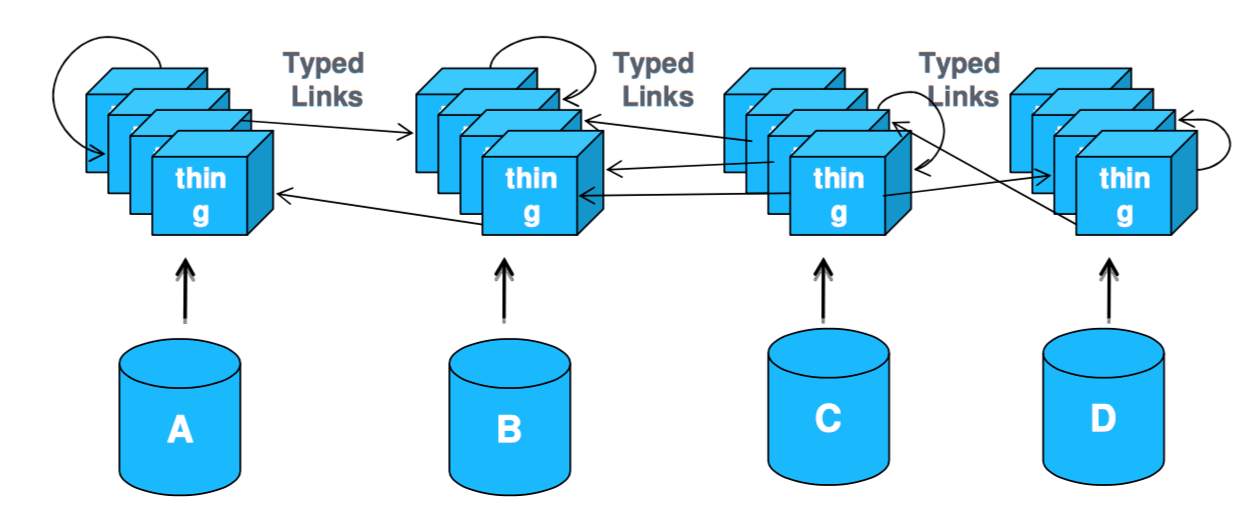
\includegraphics[width=\textwidth]{images/dataweb}
		\caption{Data-oriented web}
		\label{fig:dataweb}
	\end{figure}
\end{frame}

\begin{frame}
	% https://en.wikipedia.org/wiki/Semantic_Web#Challenges
	\begin{block}{}
		The main challenges that automated reasoning systems will have to deal in order to deliver on the promise of the Semantic Web are:
		\begin{itemize}
			\item Vastness
			\item Vagueness
			\item Uncertainty
			\item Inconsistency
			\item Deceit
		\end{itemize}
	\end{block}
	The most used solution for Semantic Web are \alert{Ontologies} (W3C).
\end{frame}